\documentclass[a0,portrait]{lab-poster}

\usepackage[brazil]{babel}    % Configuração de Linguagem (comentar para inglês)
% \renewcommand{\tablename}{Tabela}
% \renewcommand{\figurename}{Figura}

% \newcommand\itemadjust{\itemsep.5em \parskip0pt \parsep0pt}

\title{Mapeamento de recursos sob computação em névoa}
\author{Felipe Brizola Bergues Duro}
\major{Ciência da Computação}
% \major{Ciência da Computação/Engenharia da Computação/Engenharia Elétrica/...}
\advisor{Prof. Dr. Sérgio Johann Filho}

\themecolor{NavyBlue}
\unilogo{fig/ep-logo.pdf}
\lablogo{fig/ep-logo.pdf}

\begin{document}
\maketitle

%---------------------------------------------------------------

\begin{multicols}{2} 
%---------------------------------------------------------------
%	MOTIVAÇÃO
%---------------------------------------------------------------
% \color{NavyBlue}
\section*{Introdução}
% \color{Black}
\Large
\justifying
\begin{itemize}

\item A computação em névoa é um termo relativamente novo e teve sua primeira definição, dada pela Cisco Systems em 2012, como uma extensão do paradigma de computação em nuvem que provê armazenamento, computação e serviços de rede entre dispositivos finais e os servidores na nuvem \cite{DBLP:journals/corr/RomanLM16}.
\item A computação em névoa tornou-se um paradigma próprio deixando de ser um apêndice da computação em nuvem. Deste novo paradigma surgiu o termo de \textit{fog node}, que abrange desde dispositivos finais com baixa capacidade computacional até servidores poderosos na nuvem.
\item Os problemas referentes à padronização, descoberta e sincronização são os motivadores deste trabalho, uma vez que atualmente não existem mecanismos no qual um membro da névoa, seja ele um dispositivo com limitações de memória e processamento ou um computador, mapeiem os recursos disponíveis e divulgue os seus na rede.
\item Para que este objetivo fosse atingida, foi construído um protocolo de rede simples que execute em redes locais e que atue de maneira automatizada e desentralizada no processo de descobrimento e sincronização de recursos.
\item Em uma abordagem bottom-up, podemos descrever a arquiterura da computação em névoa como um conjunto de edge devices, que se comunicam com os fog nodes, e esses com servidores centrais.
Entretanto, a comunicação entre os fog nodes e os servidores centrais nao é essencial para a execução dos serviços em névoa.
\item Abaixo, está representado este conceito de computação em névoa.


\begin{center}
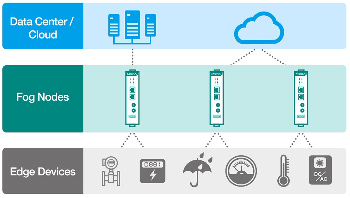
\includegraphics[width=0.75\linewidth]{fig/fig1.pdf}
\end{center}


\item A comunicação entre os \textit{fog nodes} e seus sensores, comumente chamados de \textit{edge devices}, ocorre utilizando o protocolo CoAP - Constrained Application Protocol.

% \item Especificado pela RFC-7252, o CoAP foi projetado para aplicações máquina-a-máquina e tem como foco a transferência de documentos web entre nodos com recursos limitados em redes de baixa qualidade.

% \item O modelo de interação cliente/servidor é o padrão adotado pelo CoAP, entretanto, o fato do protocolo ter sido projetado para aplicações máquina-a-máquina faz com que os dispositivos comumente desempenhem o papel de cliente e servidor simultaneamente.


% \item Segundo a RFC-6690, o Constrained RESTful Environments (CoRE) Link Format, possui como finalidade a realização de REST em nodos com recursos limitados, sendo tal característica importante em aplicações máquina-a-máquina.

% \item Um aspecto relevante ao CoRE, e de suma importancia para aplicações maquina- a-maquina, é o fato de possuir como URI padrão o prefixo /.well-known/core , definido na RFC-5785. Este prefixo é utilizado para que o servidor exponha suas políticas e recursos disponíveis.

\item explicar o impacto disso, acessar recursos de outros nodes, manter o mapeamento de recursos, etc...

\end{itemize}

\section*{\huge Protocolo Proposto}

\Large
\justifying
\begin{itemize}

% \item A imagem abaixo ilustra a pilha de protocolos utilizados na implementação deste projeto, bem como o detalhamento estrutural do protocolo proposto, intitulado Resource Mapping.

\begin{center}
	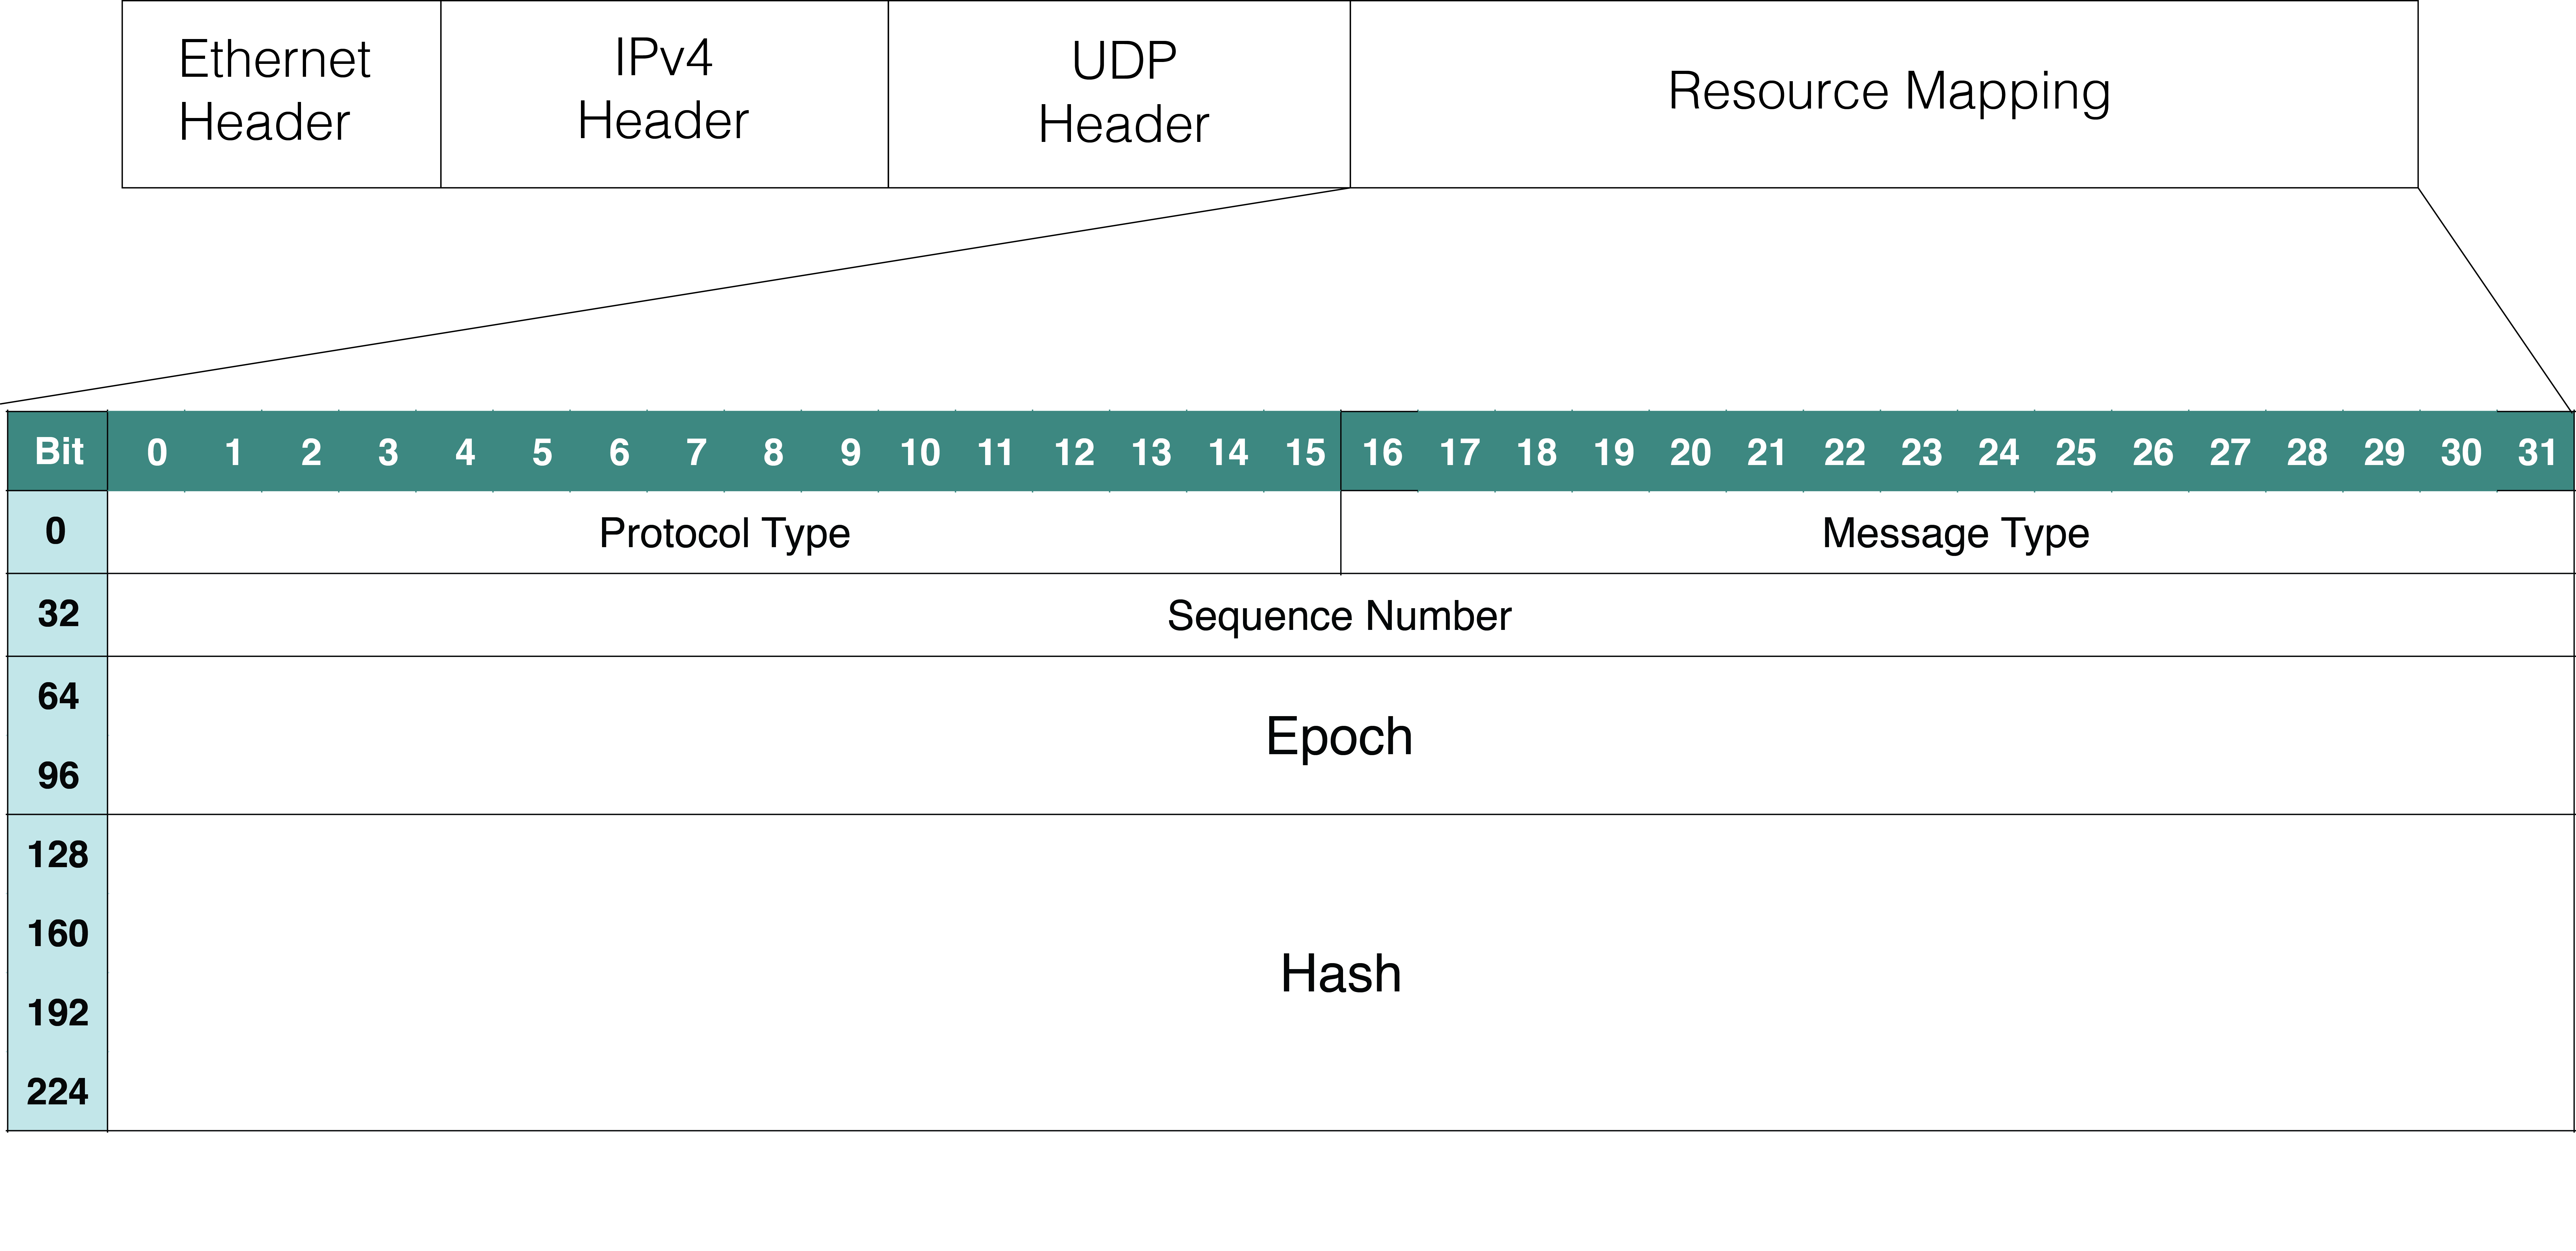
\includegraphics[width=0.9\linewidth]{fig/fig2.png}
	\end{center}

\item O campo Protocol Type é reservado para indicar a forma de encapsulamento do pacote.
\item Atualmente existem dois tipos de Messages Types possíveis, keep alive e acknowledgement.
\item Sequence Number tem o intuito de identificar o pacote enviado.
\item O campo Epoch é utilizado para indicar alterações nos recursos providos pelo fog node.
Sendo assim, quando um recurso é adicionado ou removido de um fog node, o campo Epoch é acrescido em uma unidade.
\item Por fim, o campo Hash valida a integridade dos demais campos contidos no pacote.



% \item Os fog nodes, a cada trinta segundos, enviam mensagens por multicast indicando que ainda estão em operação.
% Essas mensagens são do tipo keep alive e, portanto, fazem uso do campo Message Type.

% \item Quando as mensagens de keep alive são recebidas, é 


\end{itemize}
%---------------------------------------------------------------
%	AgentSpeak(L)
%---------------------------------------------------------------
\section*{\huge Experimentos}



%---------------------------------------------------------------
%	REFERENCES
%---------------------------------------------------------------
% Descomentar abaixo caso queira usar referências bibliográficas no poster
\vspace{-10mm}
\large
\color{NavyBlue}
\color{Black}
\raggedright
\bibliographystyle{plain}
\bibliography{poster}

\end{multicols}

%----------------------------------------------------------------------------------------
\end{document}